\documentclass[a4paper,11pt]{article}
\usepackage[utf8]{inputenc}
\usepackage[ngerman]{babel}
\usepackage{amsmath}
\usepackage{amssymb}
\usepackage{geometry}
\usepackage{graphicx}
\usepackage{wrapfig}
\usepackage{multicol}
\usepackage{float}
\usepackage{listings}
\usepackage{color}

\geometry{top=2cm, left=3cm, right=3cm, bottom=2cm}
\parindent 0pt
\setlength{\parskip}\medskipamount
\lstset{tabsize=2}
\lstset{language=Python, tabsize=4}

\title{\vspace{-1.5cm} ALP III: Aufgabenblatt 14, Übungsgruppe 1.8 }
\author {Tobias Lohse, Marvin Kleinert, Anton Drewing}
\date{\today}

\begin{document}

\maketitle

\section*{Aufgabe 1}

\subsection*{a)}
HK: \textbf{gegeben}: Graph $(V,E)$, \textbf{gesucht}: Hamiltonkreis der Länge $k$

TSP: \textbf{gegeben}: gewichteter Graph $(V,E,c)$, \textbf{gesucht}: Rundreise $R\subseteq E$ mit Kosten $k$

Wir zeigen zunächst HK $\leq_P$ TSP. Dafür konstruieren wir $f\big((V,E)\big) = (V,E',c)$ wobei $E'$ vollständig ist und $c_{ij} = 1 \Leftrightarrow (i,j)\in E$ und $c_{ij} = 2 \Leftrightarrow (i,j)\notin E$. Wenn $(V,E)$ nun einen Hamiltonkreis der Länge $k$ hat, so ergibt dieser eine Rundreise mit Kosten $k$ auf $(V,E',c)$. Falls es keinen Hamiltonkreis gibt, so muss die Rundreise mindestens einen Weg mit Kosten 2 enthalten und hat somit insgesamt Kosten $>k$, also ist auch $TSP$ nicht lösbar. 

TSP-Opt: \textbf{gegeben}: Graph $(V,E,c)$, \textbf{gesucht}: Rundreise $R\subseteq E$ mit minimalen Kosten. 

Sei $tsp\big(G=(V,E,c),k\big)$ der Algorithmus, welcher TSP entscheidet. Wir konstruieren nun zunächst einen Algorithmus $tsp\_min(G)$, welcher die geringsten Kosten auf $G$ findet. Dieser läuft wir folgt ab: 
\begin{itemize}
\item Berechne $K=\sum_{i,j} c_{ij}$.
\item Führe eine Binärsuche aus, wobei $k_o$ die obere Schranke, $k_u$ die untere Schranke und $k_m=k_o-k_u/2$ den testwert bezeichnen. 
\item Initialisiere $k_u=0$, $k_o=K$.
\item Wenn $tsp(G,k)$ wahr ist, setze $k_o=k_m$, sonst setze $k_u=k_m$.
\item Wenn $k_o=k_u=l_m$ ist, haben wir die Strecke mit geringsten Kosten gefunden.
\end{itemize}

Nun müssen wir noch die Strecke mit diesen geringsten Kosten $k_m$ finden. Dazu konstruieren wir folgenden Algorithmus $tsp\_opt$: 

\begin{itemize}
\item Setze $R=E$.
\item Für jede Kante $e$ in $R$, teste ob $tsp\_min\big((V,R\setminus\{e\}\big) = k_m$, wenn ja setze $R=R\setminus\{e\}$. 
\item Am Ende enthält $R$ alle Kanten der Rundreise. 
\end{itemize}

Wir sehen, dass $tsp\_min$ $\log\,K$-mal $tsp$ aufruft und $tsp\_opt$ $|E|$-mal $tsp_min$ aufruft. Somit haben wir gezeigt, dass HK $\leq_P$ TSP $\leq_P$ TSP-Opt, und damit gilt TSP-Opt ist ebenfalls $\mathcal{NP}$-Schwer. 

\subsection*{b)}
Wir bezeichnen mit $approx\_tsp(G)$ den $\alpha$-Appoximationsalgorithmus, welcher eine Rundreise $R$ berechnet, deren kosten höchstens $\alpha$ mal so groß wie die Kosten der optimalen Rundreise $R_{opt}$ sind: $c(R) \leq \alpha\cdot c(R_{opt})$.

Mithilfe dieses Algorithmus, konstruieren wir nun einen Algorithmus $hk(G)$, welcher für einen Graphen $G=(V,E)$ entscheidet, ob er einen Hamiltonkreis enthält. 

\begin{itemize}
\item Konstruiere den gewichteten Graphen $G'=(V,E',c)$, wobei $E'$ vollständig ist und wenn $(i,j)\in E$ ist $c_{ij}=0$ und sonst $c_{ij} = 1$. 
\item Führe $approx\_tsp(G')$ aus und erhalte eine Rundreise $R$. Sind die Kosten dieser Rundreise  gleich $c(R)=0$, so gibt es einen Hamiltonkreis, sonst nicht. 
\end{itemize}

Dieser Algorithmus funktioniert, da falls ein Hamiltonkreis existiert $c(R_{opt})$ in $G'$ immer 0 ist, wobei $R_{opt}$ der Hamiltonkreis ist. Der Approximationsalgorithmus findet somit eine Route $R$ mit $0 \leq c(R) \leq \alpha\cdot c(R_{opt}) = 0$, also findet er die optimale Route. Wenn kein Hamiltonkreis existiert, muss es in $R_{opt}$ mindestens einen Weg $(k,l)\in R_{opt}$ geben mit $c_{k,l} = 1$, also git $c(R_{opt})\geq 1$. Somit sind die Kosten der Route des durch den Approximationsalgorithmus berechneten Route $R$, beschränkt durch $1\leq c(R_{opt})\leq c(R)\leq\alpha\cdot c(R_{opt})$, damit folgt, dass $c(R) \geq 1$, falls es keinen Hamiltonkreis gibt. 

Wir betrachten nun die Laufzeit von $hk$: Die Konstruktion von $G'$ geschieht in $\mathcal{O}(|E'|)=\mathcal{O}(|V|^2)$, da nur $c$ konstruiert werden muss und $E'$ vollständig ist. Danach führt der Algorithmus nur $approx\_tsp$ aus; wenn dieses nun in $\mathcal{P}$ liegt, so liegt auch $hk$ in P. Wir wissen aber, dass HK $\mathcal{NP}$-Vollständig ist. Das heißt alle Probleme in $\mathcal{NP}$, lassen sich auf HK reduziere. Wenn dieses also in $\mathcal{NP}$ liegt, so liegen alle Probleme in $\mathcal{NP}$ in $\mathcal{P}$. Es würde gelten $\mathcal{NP}=\mathcal{P}$.

\subsection*{c)}
Wir formalisieren das Scheduling-Problem (SHED) auf zwei Maschienen, welche $n$ Operationen in einer Zeitspanne $\leq T$ ausführen sollen zunächst.

SHED: \textbf{gegeben}: Menge von Zeiten $U=\{t_1,\cdots,t_n\}$, Grenzzeit $T$, \textbf{gesucht}: Partition von $U$ in $X\subseteq U$ und $Y = U\setminus X$, so dass $\max\big(\sum_{t_i\in X}t_i\big|\sum_{t_j\in Y}t_j\big)\leq T$. 

Zunächst zeigen, wir dass SHED in $\mathcal{NP}$ liegt. Dazu konstruieren wir folgenden Algorithmus mit polynomieller Laufzeit, der bei Eingabe einer Zeit Mengen $U$ und einer Grenzzeit $T$, und einer Partition $X$ und $Y$ testet, ob diese der SHED Bedingung genügen. 

\begin{itemize}
\item Teste ob $X\subseteq U$ und $Y = U\setminus X$.
\item Teste ob $\sum_{t_i\in X}t_i\leq T$ und $\sum_{t_j\in Y}t_j\leq T$.
\item Wenn beide tests bestanden wurden, ist $(U,T,X,Y)$ eine Lösung von SHED.
\end{itemize}

Der erste Test muss alle Elemente von $U$ einmal mit den Elementen in $X$ und $Y$ vergleichen. Der zweite Test muss alle Elemente in $X$ und $Y$ einmal summieren. Somit liegt die Laufzeit in $\mathcal{O}(|U|)$, also liegt . Um zu zeigen, dass SHED $\mathcal{NP}$-schwer ist, reduzieren wir PARTITION auf SHED. 

PARTITION: \textbf{gegeben}: Zahlenmenge $A=\{a_1,\cdots a_n\}$, \textbf{gesucht}: Teilmenge $H\subseteq A$, so dass $\sum_{a_i\in H}a_i=\sum_{a_j\in U\setminus A}a_j$.

Wir konstruieren folgende Funktion $f: PARTITION \to SHED$, mit $f(A) = (A,s)$ mit $s=\sum_{a_i\in A}/2$. Wenn $A$ in Partition liegt, so gilt, dass $\exists H\subseteq A: \sum_{a_i\in H}a_i = \sum_{a_j\in A\setminus H}a_j$. Da nun aber $\sum_{a_i\in H}a_i+\sum_{a_j\in A\setminus H}a_j = \sum_{a_i\in A} = 2s$, folgt, dass $\sum_{a_i\in H}a_i= s$. Somit gibt es in $(A,s)$ eine Partition in $X=H$ und $Y=A\setminus H$, welche in SHED liegt. 

Wenn es aber keine Partition in $A$ gibt, so findet sich auch für SHED keine Partitionen. Denn nehmen wir an, wir haben eine beliebige Partition $X$ gefunden, für die $\sum_{a_i\in X}a_i\leq s$ ist, dann gilt dass $\sum_{a_j\in A\setminus X}a_j = \sum_{a_i\in A}a_i - \sum_{a_j\in X}a_j = 2s - \sum_{a_j\in X}a_j \geq s$. Da es nun aber nicht sein kann, dass $\sum_{a_i\in X}a_i = \sum_{a_j\in A\setminus X}a_j = s$, da sonst PARTITION gelöst würde, so ist die Summe über alle $Y=A\setminus X$ also $\sum_{a_j\in Y}a_j > s$ und somit ist das Wort auch nicht in SHED. Damit Haben wir gezeigt, dass SHED in $\mathcal{NP}$ ist und $\mathcal{NP}$-schwer ist, ist SHED also auch $\mathcal{NP}$-Vollständig. \\


\section*{Aufgabe 2}

\subsection*{a) \hspace{4.5cm} b) \vspace{-0.4cm}}
\begin{figure}[h]
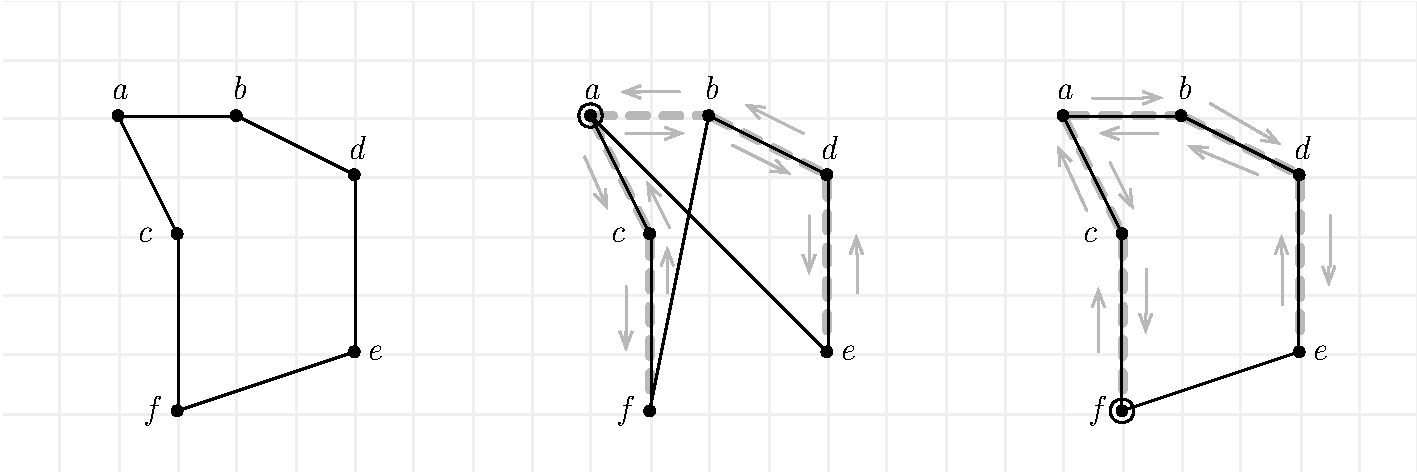
\includegraphics[width=\textwidth]{a2.pdf}
\end{figure}

Die kürzeste Rundreise hat eine Länge von $2+\sqrt 5+3+\sqrt{10}+3+\sqrt 5 \approx 15,63$. Wenn wir mit dem minimalen Spannbaum (grau gestrichelt) und Tiefensuche approximieren, dann hängt das Ergebnis vom Startknoten ab. Starten wir in Knoten $a$, so erhalten wir als Rundreise $a-c-d-b-d-e-a$, mit einer Länge von $\sqrt 5+3+\sqrt{26}+\sqrt 5+3+\sqrt{32}\approx 21,23\leq 2\cdot 15,63$. Wenn wir in $f$ starten, so erhalten wir auch mit der Approximation die kürzeste Rundreise. \\


\section*{Aufgabe 3}

\subsection*{a)}
Wenn wir zwei Knoten nehmen, die miteinander verbunden sind $G=\big(\{1,2\},\{(1,2)\}\big)$, so gibt der Approximationsalgorithmus als überdeckende Knotenmenge $\{1,2\}$ zurück. Die minimale überdeckende Knotenmenge wäre aber nur $\{1\}$ oder $\{2\}$.

\subsection*{b)}
Der folgende Algorithmus \lstinline|sat_dnf| gibt an, ob ein boolscher Term in DNF-Form erfüllbar ist. Dabei geht er im schlimmsten Fall jedes Literal einmal durch und testet es gegen einen gespeicherten Wert in einem Wörterbuch. Bei insgesamt $n$ Literalen in allen Klauseln der DNF liegt die Laufzeit somit in $\mathcal{O}(n)$ und somit gilt \lstinline|sat_dnf|$\in\mathcal{P}$.

\begin{lstlisting}
def sat_dnf(DNF):
	found = False
	Klausel = DNF.first_Klausel
	while Klausel != null and not found:
		V = {}
		found = True
		for Literal in Klausel:
			if Literal not in V:
				V[Literal] = Literal.Wert
			else:
				if V[Literal] != Literal.Wert:
					found = False
					break
		Klausel = DNF.next_Klausel
	return found
\end{lstlisting}

\subsection*{c)}

Wir konstruieren einen Algorithmus \lstinline|sat_bel| der eine erfüllende Belegung für eine Aussage konstruiert und dabei auf den Algorithmus \lstinline|sat| zuückgreift, welcher SAT entscheidet: 

\begin{lstlisting}
def sat_bel(Aussage):
	if not sat(Aussage):
		raise Exception("not satisfiable")
	B = {}
	for Literal in Aussage:
		Aussage.replace_each(Literal, True)
		B[Literal] = True
		if not sat(Aussage_cp):
			Aussage.replace_each(Literal, False)
			B[Literal] = False
	return B
\end{lstlisting}

Dabei ersetzt \lstinline|replace_each(Literal, Wert)| alle vorkommen von Literal in Aussage durch Wert. Wenn die Aussage erfüllbar ist, gehen wir also Literal für Literal durch und legen es auf einen Wert fest, unter dem die Aussage noch erfüllbar ist. Am Ende haben wir eine Belegung gefunden, unter welcher die Aussage erfüllbar ist. 

Wenn nun $a$ die Anzahl der literalen Therme in der Aussage ist und $n$ die Anzahl der verschiedenen Literale ist, so ergibt sich für die Laufzeit $T(\text{replace\_each}) = a$. Damit ist die Laufzeit von $T(\text{sat\_bel}) = n\cdot\big(a+T(\text{sat})+1\big)$. Wenn nun SAT$\in\mathcal{P}$ ist, folgt mit $n\leq a$, dass unser Algorithmus auch polynomielle Laufzeit hat.





\end{document}